
\begin{tikzpicture}
    \node [examplebox] (box){
        \begin{minipage}{0.475\textwidth}
            { Aging-Time: $50$ Sekunden}
            \\
            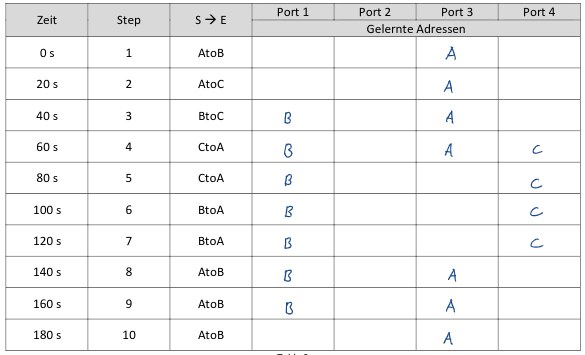
\includegraphics[scale=0.55]{img/filteringdb.png}
        \end{minipage}
    };
    \node[exampletitle, right=8pt] at (box.north west) {Filtering-Database};
\end{tikzpicture}

\begin{tikzpicture}
    \node [examplebox] (box){
        \begin{minipage}{0.475\textwidth}
            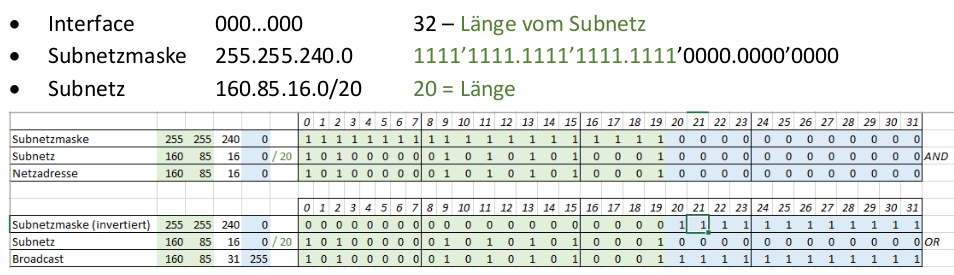
\includegraphics[scale=0.4]{img/ipaddressierung.png}
        \end{minipage}
    };
    \node[exampletitle, right=8pt] at (box.north west) {Addressierung IPv4 Beispiel:};
\end{tikzpicture}

\begin{multicols*}{2}
    \begin{tikzpicture}
        \node [examplebox] (box){
            \begin{minipage}{0.2125\textwidth}


                \unsignedbytecalc{177}

            \end{minipage}
        };
        \node[exampletitle, right=8pt] at (box.north west) {Umrechnung Dezimal zu Binär};
    \end{tikzpicture}


    \begin{tikzpicture}
        \node [examplebox] (box){
            \begin{minipage}{0.2125\textwidth}
                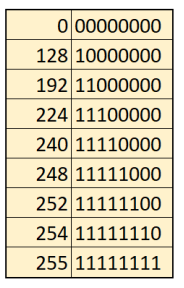
\includegraphics[scale=0.4125]{img/binary-subnet.png}

            \end{minipage}
        };
        \node[exampletitle, right=8pt] at (box.north west) {Umrechungstabelle};
    \end{tikzpicture}

\end{multicols*}


\begin{tikzpicture}
    \node [examplebox] (box){
        \begin{minipage}{0.475\textwidth}
            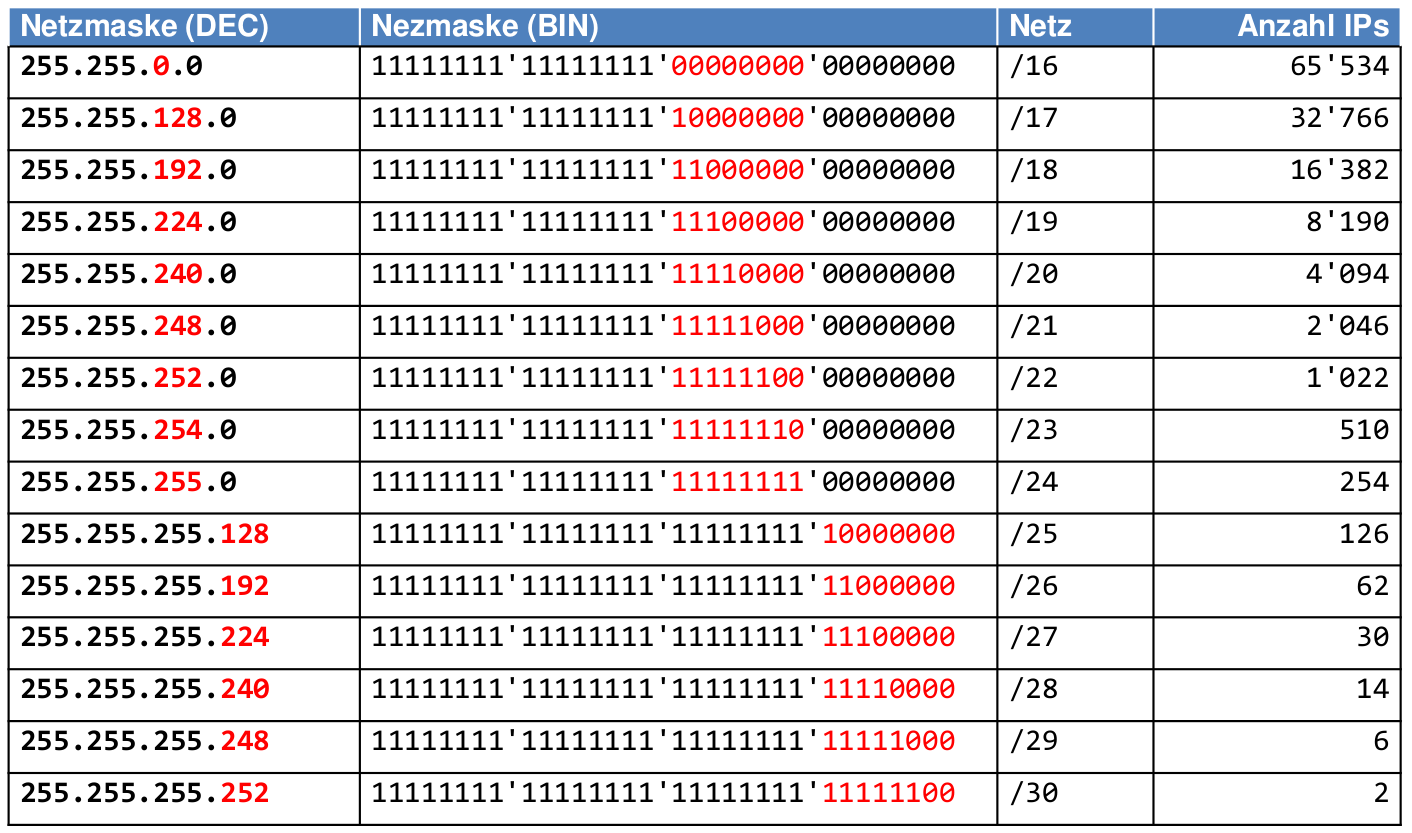
\includegraphics[scale=0.265]{img/subnetzmasken.png}
        \end{minipage}
    };
    \node[exampletitle, right=8pt] at (box.north west) {IP Subnetzmasken};
\end{tikzpicture}
\begin{tikzpicture}
    \node [examplebox] (box){
        \begin{minipage}{0.475\textwidth}
            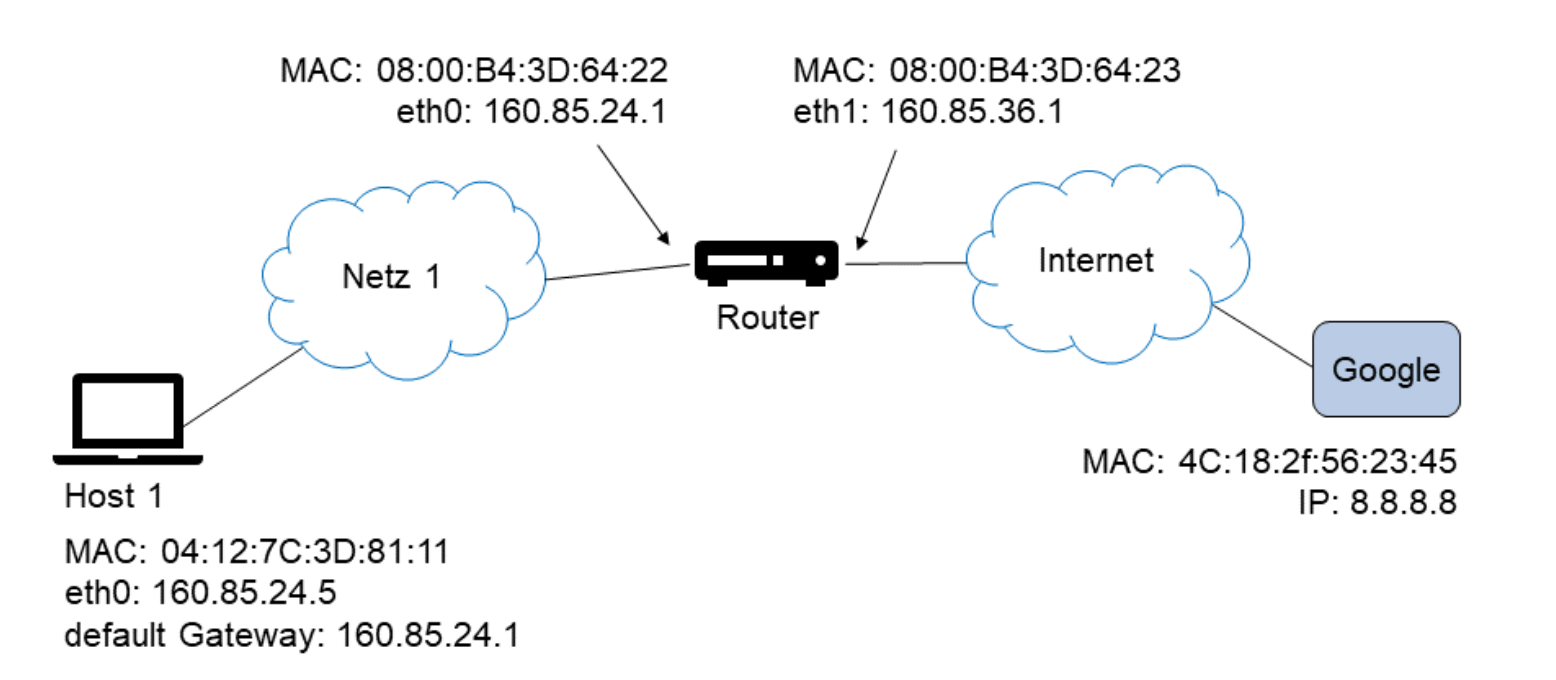
\includegraphics[scale=0.2125]{img/arp_example.png}
            \\
            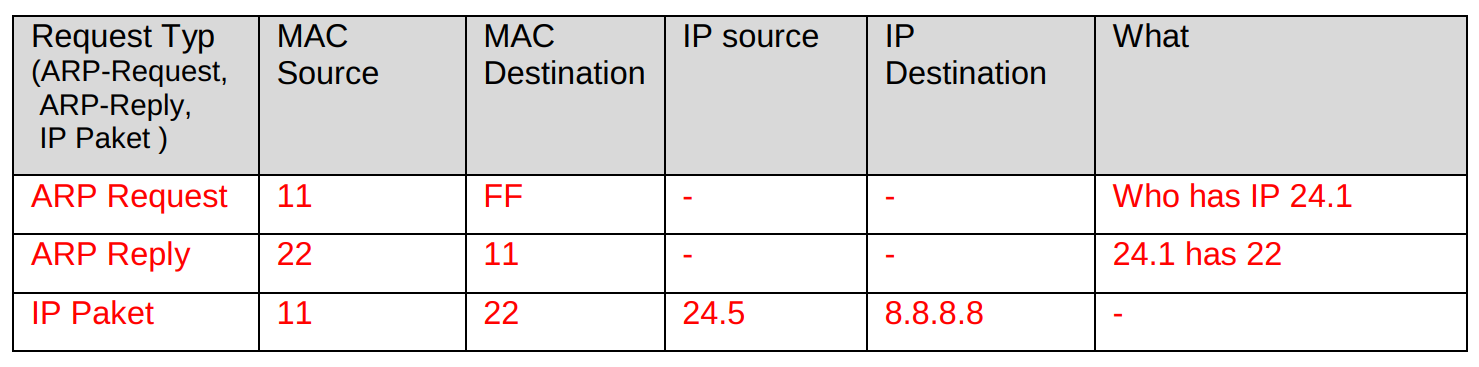
\includegraphics[scale=0.25]{img/arp_example_sol.png}
        \end{minipage}
    };
    \node[exampletitle, right=8pt] at (box.north west) {ARP Table Beispiel};
\end{tikzpicture}


\begin{tikzpicture}
    \node [examplebox] (box){
        \begin{minipage}{0.475\textwidth}

            Gegeben ist das Netz 172.30.10.0/25. Dieses Netz soll in drei Subnetze aufgeteilt werden: ein größeres Subnetz 1 für 50 IP-Hosts und zwei kleinere Subnetze 2 und 3 für je 25 IP-Hosts.

            \begin{enumerate}
                \item \textbf{Subnetz 1 für 50 Hosts:}

                      Wir benötigen 6 Bits für die Host-IDs, um mindestens 50 Hosts zu unterstützen (2\^6 - 2 = 62). Das führt zu einer Subnetzmaske von /26 (32 - 6 = 26).

                      \begin{itemize}
                          \item Netzadresse: 172.30.10.0/26
                          \item Broadcastadresse: 172.30.10.63/26
                          \item Anzahl adressierbarer Hosts: 62
                      \end{itemize}

                \item \textbf{Subnetz 2 und 3 für jeweils 25 Hosts:}

                      Wir benötigen 5 Bits für die Host-IDs, um mindestens 25 Hosts zu unterstützen (2\^5 - 2 = 30). Das führt zu einer Subnetzmaske von /27 (32 - 5 = 27).

                      \begin{itemize}
                          \item \textbf{Subnetz 2:}
                                \begin{itemize}
                                    \item Netzadresse: 172.30.10.64/27
                                    \item Broadcastadresse: 172.30.10.95/27
                                    \item Anzahl adressierbarer Hosts: 30
                                \end{itemize}

                          \item \textbf{Subnetz 3:}
                                \begin{itemize}
                                    \item Netzadresse: 172.30.10.96/27
                                    \item Broadcastadresse: 172.30.10.127/27
                                    \item Anzahl adressierbarer Hosts: 30
                                \end{itemize}
                      \end{itemize}
            \end{enumerate}

        \end{minipage}
    };
    \node[exampletitle, right=8pt] at (box.north west) {Subnet Beispiel 1};
\end{tikzpicture}


\begin{tikzpicture}
    \node [examplebox] (box){
        \begin{minipage}{0.475\textwidth}

            Sie bekommen von Ihrem Internet Service Provider (ISP) ein privates Klasse-C Netz zugeteilt. In Ihrem Haus befinden sich 4 Parteien, welche sich den Internet-Anschluss teilen. Sie geben jeder Partei ein gleich grosses Subnetz, indem sie das Klasse-C Netz 192.168.1.0/24 in 4 Subnetze aufteilen.

            Wir teilen das gegebene Klasse-C Netz 192.168.1.0/24 in vier gleich große Subnetze auf, indem wir zwei zusätzliche Bits für die Subnetz-ID verwenden. Dies führt zu einer neuen Subnetzmaske von /26 und 62 adressierbaren Hosts pro Subnetz ($2^6 - 2 = 62$).

            \begin{enumerate}
                \item \textbf{Subnetz 1:}
                      \begin{itemize}
                          \item Netzadresse: 192.168.1.0/26
                          \item Netzmaske: 255.255.255.192
                          \item Broadcastadresse: 192.168.1.63/26
                          \item Default Gateway: 192.168.1.1
                          \item Anzahl adressierbarer Hosts: 62
                      \end{itemize}

                \item \textbf{Subnetz 2:}
                      \begin{itemize}
                          \item Netzadresse: 192.168.1.64/26
                          \item Netzmaske: 255.255.255.192
                          \item Broadcastadresse: 192.168.1.127/26
                          \item Default Gateway: 192.168.1.65
                          \item Anzahl adressierbarer Hosts: 62
                      \end{itemize}

                \item \textbf{Subnetz 3:}
                      \begin{itemize}
                          \item Netzadresse: 192.168.1.128/26
                          \item Netzmaske: 255.255.255.192
                          \item Broadcastadresse: 192.168.1.191/26
                          \item Default Gateway: 192.168.1.129
                          \item Anzahl adressierbarer Hosts: 62
                      \end{itemize}

                \item \textbf{Subnetz 4:}
                      \begin{itemize}
                          \item Netzadresse: 192.168.1.192/26
                          \item Netzmaske: 255.255.255.192
                          \item Broadcastadresse: 192.168.1.255/26
                          \item Default Gateway: 192.168.1.193
                          \item Anzahl adressierbarer Hosts: 62
                      \end{itemize}
            \end{enumerate}


        \end{minipage}
    };
    \node[exampletitle, right=8pt] at (box.north west) {Subnet Beispiel 2};
\end{tikzpicture}


\begin{tikzpicture}
    \node [examplebox] (box){
        \begin{minipage}{0.475\textwidth}
            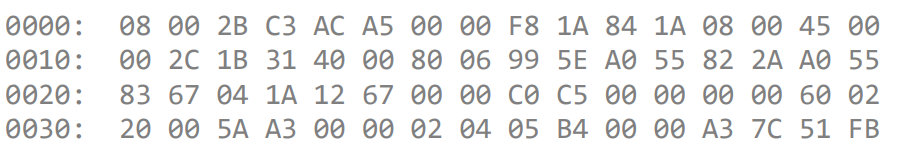
\includegraphics[scale=0.4]{img/wireshark.png}

            \begin{itemize}[noitemsep]
                \item  Oktett 0-5: Destination MAC-Address
                \item  Oktett 6-11: Source MAC-Address
                \item  Oktett 12/13: Length / Type → hier Type = 0x0800
                \item   Oktett 14-59: Data / padding
                \item   Oktett 60-63: Frame Check Sequence
            \end{itemize}

            $$\text{3. Oktett} = 0x2B = 00101011$$
        \end{minipage}
    };

    \node[exampletitle, right=8pt] at (box.north west) {
        Wireshark Hex-Dump};
\end{tikzpicture}

\begin{tikzpicture}
    \node [examplebox] (box){
        \begin{minipage}{0.475\textwidth}


            \begin{center}
                \begin{tabular}{| >{\centering\arraybackslash}m{1in} | >{\centering\arraybackslash}m{1in} | >{\centering\arraybackslash}m{1in} |}
                    \hline
                    \textbf{Dezimal} & \textbf{Hexadezimal} & \textbf{Binär} \\
                    \hline
                    0                & 0                    & 0000           \\
                    \hline
                    1                & 1                    & 0001           \\
                    \hline
                    2                & 2                    & 0010           \\
                    \hline
                    3                & 3                    & 0011           \\
                    \hline
                    4                & 4                    & 0100           \\
                    \hline
                    5                & 5                    & 0101           \\
                    \hline
                    6                & 6                    & 0110           \\
                    \hline
                    7                & 7                    & 0111           \\
                    \hline
                    8                & 8                    & 1000           \\
                    \hline
                    9                & 9                    & 1001           \\
                    \hline
                    10               & A                    & 1010           \\
                    \hline
                    11               & B                    & 1011           \\
                    \hline
                    12               & C                    & 1100           \\
                    \hline
                    13               & D                    & 1101           \\
                    \hline
                    14               & E                    & 1110           \\
                    \hline
                    15               & F                    & 1111           \\
                    \hline
                \end{tabular}
            \end{center}


        \end{minipage}
    };
    \node[exampletitle, right=8pt] at (box.north west) {
        Dezimal, Hexadezimal, Binär};
\end{tikzpicture}


\begin{tikzpicture}
    \node [examplebox] (box){
        \begin{minipage}{0.475\textwidth}
            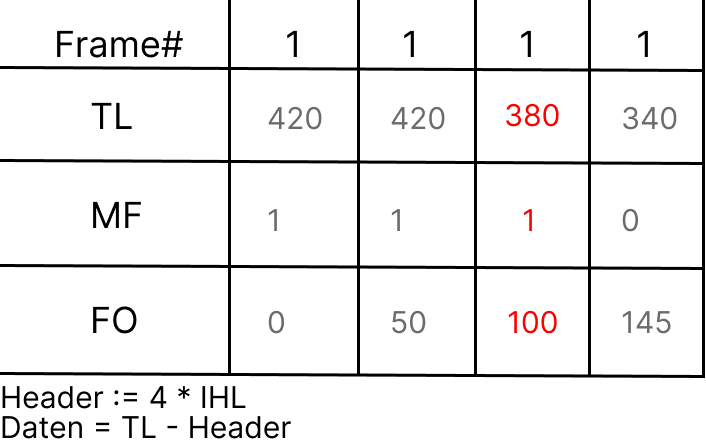
\includegraphics[scale=1]{img/Group 7_x3.png}
            \\
            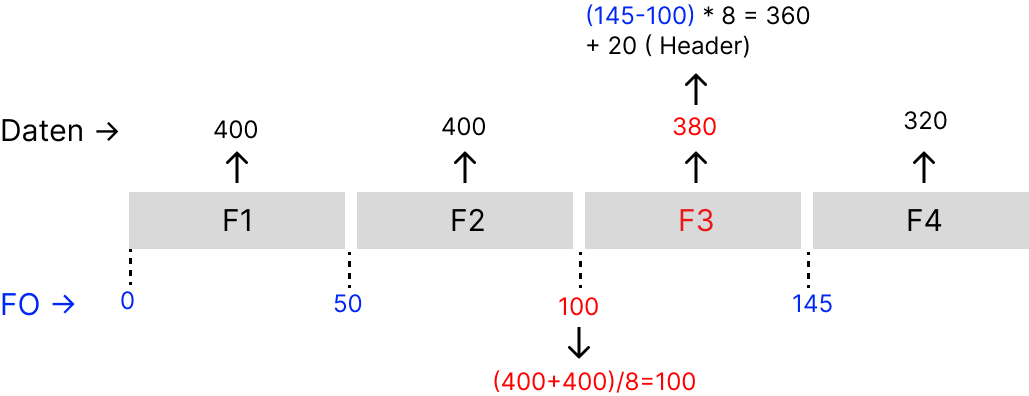
\includegraphics[scale=1.1125]{img/Group 6_x3.png}


        \end{minipage}
    };
    \node[exampletitle, right=8pt] at (box.north west) {
        Fragmentierung};
\end{tikzpicture}